% \frame{
%     \frametitle{\ex{``Classical'' MS/MS spectra based metabolite identification}}
%     
% \begin{figure}[t]
%     \centering
%     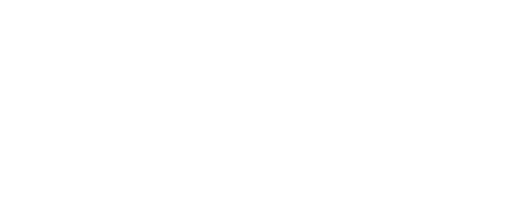
\includegraphics[width=1.0\textwidth]{images/molecular_candidates_only_iokr.pdf}
% \end{figure}    
% }
% 

\frame{
    \frametitle{Predicted retention orders for metabolite identification} 
%     \framesubtitle{Exploit observed retention order in complex LC-MS experiment}
    
\begin{figure}[t]
    \centering
    \includegraphics[width=0.8\textwidth]{images/lcms_spectrum_complex_small.pdf}
\end{figure}
\vspace{-0.15cm}
\begin{small}
\begin{block}{Identification workflow}
\vspace{-0.15cm}
\begin{enumerate}
    \item execute 1. (query candidates) and 2. (predict matching scores)
    \item Construct a layered graph:
\begin{itemize}
    \item Nodes: Molecular candidate structures $m_{i,j}$
    \item Edges: Encode matching scores and predicted retention orders   
\end{itemize}

    
%     where the nodes are molecular candidates and the edges encode the MS/MS matching scores as well as the predicted retention order.
%     \item Predict retention orders between all candidates $m_{i,j}$ and $m_{i+1,s}$ of MS/MS spectra of consecutively eluting molecules. \hfill\ex{$x_1$ and $x_2$}
    \item Find the \emph{overall} most consistent metabolite identification using the shorest path algorithm.
\end{enumerate}
\end{block}
\end{small}
}

\frame{
    \frametitle{\ex{Predicted retention orders for metabolite identification}} 
    
\only<1>{
\begin{figure}[c]
    \centering
    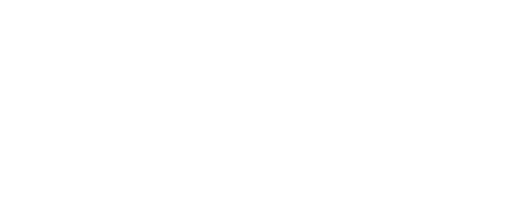
\includegraphics[width=0.9\textwidth]{images/molecular_candidates_no_shortest_path.pdf}
\end{figure}
}
\only<2>{
\begin{figure}[c]
    \centering
    \includegraphics[width=0.9\textwidth]{images/molecular_candidates.pdf}
\end{figure}
}
\vspace{-0.15cm}
\begin{small}
\begin{itemize}
    \item<1-> Edges connecting candidates of consecutive layers with edge weight:
\vspace{-0.25cm}
\begin{equation}
    \delta_{(i,j),(i+1,s)}=-y_{i+1,s}+D\cdot\max(0,\underbrace{\VEC{w}^T(\phi(m_{i,j})-\phi(m_{i+1,s})}_{\text{\alert<1>{RankSVM order penalty}}})),
\end{equation}
    $D\geq0$ weight on order penmalty: $\max(\ldots)>0$ if observed $\neq$ predicted order.
    \item<2> Candidates along the \alert<2>{shortest path} from first to last layer: \emph{most consistent identification}.
\end{itemize}
\end{small}

}

% \begin{block}{Retention order prediction function using RankSVM}
% \vspace{-0.5cm}
% \begin{equation}
%     f(\mol_i = \includegraphics[scale=1.2]{images/mol_i_unknown.pdf},\mol_j = \includegraphics[scale=1.2]{images/mol_j_unknown.pdf} ) 
%         = \begin{cases}
%             1  & \mol_i = \includegraphics[scale=1.2]{images/mol_i_unknown.pdf} \text{ elutes before } \mol_j = \includegraphics[scale=1.2]{images/mol_j_unknown.pdf}\\
%             -1 & \text{otherwise}
%         \end{cases}
% \end{equation}
% \end{block}
